\documentclass[a4paper]{article}

\usepackage[english,russian]{babel}
\usepackage{hyperref}
\usepackage{filecontents}
\hypersetup{
    colorlinks,
    citecolor=black,
    filecolor=black,
    linkcolor=black,
    urlcolor=blue
}
\usepackage{listings}
\usepackage{color}
\usepackage{xcolor}
\definecolor{mygreen}{rgb}{0,0.6,0}
\definecolor{mygray}{rgb}{0.5,0.5,0.5}
\definecolor{mymauve}{rgb}{0.58,0,0.82}
\definecolor{comment}{HTML}{039699}
\definecolor{string}{HTML}{449060}
\definecolor{keyword}{HTML}{83007b}

\lstset{
linewidth=\linewidth,
  backgroundcolor=\color{white},   % choose the background color; you must add \usepackage{color} or \usepackage{xcolor}; should come as last argument
  basicstyle=\footnotesize,        % the size of the fonts that are used for the code
  breakatwhitespace=false,         % sets if automatic breaks should only happen at whitespace
  breaklines=true,                 % sets automatic line breaking
  captionpos=b,                    % sets the caption-position to bottom
  commentstyle=\color{comment},    % comment style
  deletekeywords={...},            % if you want to delete keywords from the given language
  escapeinside={\%*}{*)},          % if you want to add LaTeX within your code
  extendedchars=true,              % lets you use non-ASCII characters; for 8-bits encodings only, does not work with UTF-8
  firstnumber=0,                % start line enumeration with line 1000
  frame=single,	                   % adds a frame around the code
  keepspaces=true,                 % keeps spaces in text, useful for keeping indentation of code (possibly needs columns=flexible)
  keywordstyle=\color{keyword},       % keyword style
  language=python,                 % the language of the code
  morekeywords={*,...},            % if you want to add more keywords to the set
  numbers=left,                    % where to put the line-numbers; possible values are (none, left, right)
  numbersep=5pt,                   % how far the line-numbers are from the code
  numberstyle=\tiny\color{mygray}, % the style that is used for the line-numbers
  rulecolor=\color{black},         % if not set, the frame-color may be changed on line-breaks within not-black text (e.g. comments (green here))
  showspaces=false,                % show spaces everywhere adding particular underscores; it overrides 'showstringspaces'
  showstringspaces=false,          % underline spaces within strings only
  showtabs=false,                  % show tabs within strings adding particular underscores
  stepnumber=1,                    % the step between two line-numbers. If it's 1, each line will be numbered
  stringstyle=\color{string},     % string literal style
  tabsize=4,	                   % sets default tabsize to 2 spaces
  title=Реализация численного решения   % show the filename of files included with \lstinputlisting; also try caption instead of title
}

\usepackage{float}
\usepackage{subcaption}
\usepackage[utf8]{inputenc}
\usepackage[14pt]{extsizes}
\usepackage{physics}
\usepackage{graphicx}
\graphicspath{{misc/}}
\usepackage{setspace,amsmath}
\usepackage[left=20mm, top=15mm, right=15mm, bottom=15mm, nohead, footskip=10mm]{geometry} 
\usepackage[nottoc]{tocbibind}
\usepackage[backend=biber]{biblatex}
\addbibresource{lit.bib}

\begin{document} 

\begin{center}
    \hfill \break
    ФЕДЕРАЛЬНОЕ ГОСУДАРСТВЕННОЕ БЮДЖЕТНОЕ ОБРАЗОВАТЕЛЬНОЕ 

    УЧРЕЖДЕНИЕ ВЫСШЕГО ОБРАЗОВАНИЯ

    «МОСКОВСКИЙ ГОСУДАРСТВЕННЫЙ УНИВЕРСИТЕТ

    имени М.В.ЛОМОНОСОВА» 

    \hfill \break
    \normalsize{ФИЗИЧЕСКИЙ ФАКУЛЬТЕТ}\\
    \hfill \break
    \normalsize{КАФЕДРА ОБЩЕЙ ФИЗИКИ И МОЛЕКУЛЯРНОЙ ЭЛЕКТРОНИКИ}\\
    \hfill\break
    \hfill \break
    \normalsize{КУРСОВАЯ РАБОТА}\\
    \hfill \break
    \large\textbf{«ЧИСЛЕННОЕ РЕШЕНИЕ ДВУМЕРНОГО УРАВНЕНИЯ ТЕПЛОПРОВОДНОСТИ ПРИ ПОМОЩИ МЕТОДА ПЕРЕМЕННЫХ НАПРАВЛЕНИЙ»}\\
    \hfill \break

\end{center}

\begin{flushright}

    Выполнил студент:

    406 группа

    Гафни Д.

    $\underset{\text{подпись студента}}{\underline{\hspace{0.3\textwidth}}}$

    \hfill\break

    Научный руководитель:

    Приклонский В.И.

    $\underset{\text{подпись научного руководителя}}{\underline{\hspace{0.3\textwidth}}}$
    
    \hfill\break
    \hfill\break
    \hfill\break
    \hfill\break
    \hfill\break
    \hfill\break
    \hfill\break
    \hfill\break
    \hfill\break
    \begin{center}

    Москва

    \hfill\break
    2020
\end{center}
\end{flushright}

\tableofcontents

\clearpage

\section{Постановка задачи}
Используя метод переменных направлений, решить краевую задачу:

\begin{equation}
\left\{\begin{array}{l}{\frac{\partial u}{\partial t}=\Delta u+(y t)^{2}, ~~ 0<x<2, ~~ 0<y<1, ~~ t>0} \\
{\left.\frac{\partial u}{\partial x}\right|_{x=0}=\left.u\right|_{x=2}=0} \\ 
{\left.u\right|_{y=0}=\left.u\right|_{y=1}=0} \\ 
{\left.u\right|_{t=0}=\cos (\pi x / 4) \cdot y(1-y)}\end{array}\right.
\end{equation}

\section{Численное решение}
\subsection{Сетка}

Введем в расчетной области сетку, используя фиктивные узлы в окрестности границ, чтобы получить второй порядок аппроксимации для условий Неймана:

\begin{equation}
\begin{cases}
x_0=0; ~~ x_n = x_0 + n h_x, ~~ n = 0,1,..., N; ~~ x_N = 2  \longrightarrow h_x = \frac{2}{N-1}\\
y_0=0; ~~ y_m = y_0 + m h_y, ~~ m = 0,1,..., M; ~~ y_M = 1  \longrightarrow h_y = \frac{1}{M-1}\\
t_j=j\tau, ~~ j=0,1,...,J; ~~ t_J=T \longrightarrow \tau= \frac{T}{J}
\end{cases}
\end{equation}

На данной сетке будем рассматривать
сеточную функцию $w^{j}_{n,m} = u(x_n,y_m,t_j)$.

\subsection{Аппроксимация}
\subsubsection{Оператор Лапласа}

Аппроксимируем оператор Лапласа $\Delta = \frac{\partial^2 }{{\partial x}^2} + \frac{\partial^2 }{{\partial y}^2}$
разностным оператором $\Lambda w = \Lambda _x w + \Lambda _y w$, где

\begin{equation}
\begin{aligned}
\Lambda _x w = \frac{w_{n-1,m}-2w_{n,m}+w_{n+1,m}}{h_x^{2}}, \\
\Lambda _y w = \frac{w_{n,m-1}-2w_{n,m}+w_{n,m+1}}{h_y^{2}}. \\
\end{aligned} 
\end{equation}

Данное приближение имеет второй порядок аппроксимации.
Здесь и далее в соответствующих ситуациях для краткости верхний индекс j, соответствующий времени,
может быть негласно опущен, как и другие.

\subsubsection{Неоднородность}
\begin{equation}
f(y, t) = (yt)^2 \longrightarrow f^{j}_{n,m} = (m j h_y h_t)^2, \\
 ~~где ~~ m=0,1,...,M,~~ j=0,1,...,J.
\end{equation}

Неоднородность аппроксимируется точно.

\subsubsection{Начальное условие}
\begin{equation}
{\left.u\right|_{t=0}=\cos (\pi x / 4) \cdot y(1-y)} \longrightarrow w^{0}_{n,m} = \cos (\pi n h_x / 4) \cdot m h_y (1 - m h_y)
\end{equation}

Начальное условие аппроксимируется точно.

\subsubsection{Граничное условие}

\begin{itemize}
 \item По $x~$:
$~~\begin{cases}
w_{0,m} = w_{1,m}\\
w_{N,m} = 0
\end{cases}$
$~~~~~m=0,1,...,M$
\item По $y~$:
$~~\begin{cases}
w_{n,0} = 0\\
w_{n,M} = 0
\end{cases}$
$~~~~~~~~~n=0,1,...,N$
\end{itemize}

Условие при $ x=0 $ имеет первый порядок аппроксимации; остальные аппроксимируются точно.

\subsection{Метод переменных направлений}
В данном методе переход со слоя $j$ на слой $j+1$ осуществляется в два этапа, с помощью вспомогательного промежуточного слоя $j+1/2$. Схема переменных направлений безусловно устойчива при любых шагах $h_x, h_y, \tau$. При условии, что для начальных и граничных условий порядки аппроксимации будут не ниже первого, и с учетом вышеописанной аппроксимации дифференциальных операторов, которая имеет первый порядок, метод переменных направлений будет давать первый порядок аппроксимации в данном случае. Рассмотрим подробно переход со слоя $j$ на промежуточный слой $j+1/2$ и дальнейший переход с промежуточного слоя $j+1/2$ на слой $j+1$.

\subsubsection{Переход к промежуточному слою}
Пусть значения на слое $j$ уже известны (на самом первом шаге значения $w~^{0}_{n,m}$ известны из начального условия). Перейдем на вспомогательный промежуточный слой $j + 1/2$, используя \textbf{неявную схему по переменной $x$ и явную - по переменной $y$}:

\begin{itemize}
\item Заменим выражение $\frac{\partial^2 }{{\partial x}^2}$ разностным аналогом, взятым на слое $~j+1/2: ~~\Lambda _x w~^{j + 1/2}$.

\item А выражение $\frac{\partial^2 }{{\partial y}^2}$ разностным аналогом, взятым на слое $~j:~~\Lambda _y w~^j$. 
\end{itemize}

При этом неоднороднось $f(x,y,t)$ в правой части уравнения аппроксимируем на промежуточным слое $~j+1/2$. 

В результате придем к разностному уравнению: 

\begin{equation}
\frac{w~^{j+1/2}-w~^j}{0.5 \tau} = \Lambda _x w~^{j+1/2} + \Lambda _y w~^{j} + f^{j+1/2}
\end{equation}

Перейдем к конкретной задаче и добавим соответствующее граничное условие:

\begin{equation}
\begin{cases}
w~^{j+1/2}_{n,m} - w~^j_{n,m} = (~\frac{\tau}{2{h_x}^2} ~w~^{j+1/2}_{n+1, ~m}-\frac{\tau}{{h_x}^2} ~w~^{j+1/2}_{n, ~m}+\frac{\tau}{2{h_x}^2} ~w~^{j+1/2}_{n-1, ~m}~)+\\+(~\frac{\tau}{2{h_y}^2} ~w~^{j}_{n, ~m+1}-\frac{\tau}{{h_y}^2} ~w~^{j}_{n, ~m}+\frac{\tau}{2{h_y}^2} ~w~^{j}_{n, ~m-1}~)+\frac{\tau}{2}(m j h_y h_t)^2 \\
w~^{j+1/2}_{0,m} = w~^{j+1/2}_{1,m},~~~~w~^{j+1/2}_{N,m} = w~^{j+1/2}_{N-1,m}
\end{cases}
\end{equation}
 
$$
\text{~~где~~} n = 1,2, ...,N-1, ~~ m=1,2,...,M-1
$$

При каждом фиксированным $n=0,1,...,N-1$ можно переписать:

\begin{equation}
\begin{cases}
\frac{\tau}{2{h_y}^2} ~w~^{j+1}_{n,m-1} - \left(1+\frac{\tau}{{h_y}^2}\right) ~w~^{j+1}_{n,m} + \frac{\tau}{2{h_y}^2} ~w~^{j+1}_{n, ~m+1}=\\-\left[~w~^{j+1/2}_{n, ~m} + \frac{\tau}{2{h_x}^2} ~\left(w~^{j+1/2}_{n+1, ~m}-~2w~^{j+1/2}_{n, ~m}+~w~^{j+1/2}_{n, ~m}\right)+\frac{\tau}{2}(m j h_y h_t)^2 \right]\\ 
\\w~^{j+1}_{0,m} = w~^{j+1}_{1,m},~~~~w~^{j+1}_{N,m} = 0\\
\end{cases}
\end{equation}
$$
\text{~~где~~~} m=1,2,...,M-1
$$

Введем обозначения:

$\chi_n = w~^{j+1/2}_{n,m}, ~~~\chi_{n-1} = 0, ~~~\ \chi_{n+1}=w~^{j+1/2}_{n+1,m},$

$A^x=B^x=\frac{\tau}{2{h_x}^2}~, ~~~C^x=\left(1+\frac{\tau}{2{h_x}^2}\right),$

$F^x_n=~w~^{j}_{n, ~m} + \frac{\tau}{2{h_y}^2} ~\left(w~^{j}_{n, ~m+1}-~2w~^{j}_{n, ~m}+~w~^{j}_{n, ~m-1}\right)+\frac{\tau}{2}(m j h_y h_t)^2~.$

Получим простую систему, состоящую из уравнения, в котором неизвестные связаны рекуррентным соотношением, и граничных условий:

\begin{equation}
\begin{cases}
A^x \chi_{n-1} - C^x \chi_n +B^x \chi_{n+1} = -F^x_n,\\
\chi_0=\chi_1,~~~~\chi_N=\chi_{N-1}.
\end{cases}~~~~n=1,...,N-1
\end{equation}

Данную систему можно решить методом прогонки.

И снова получим простую систему уже для перехода $~j + 1/2\longrightarrow j+1$, состоящую из уравнения, в котором неизвестные связаны рекуррентным соотношением, и граничных условий:

\begin{equation}
\begin{cases}
A^y \gamma_{n-1} - C^y \gamma_n +B^y \gamma_{n+1} = -F^y_m,\\
\gamma_0=\gamma_1,~~~~\gamma_n=\gamma_{n-1}.
\end{cases}~~~~m=1,...,M-1
\end{equation}

Данная система аналогично решается методом прогонки.

\subsubsection{Метод прогонки}
Рассмотрим систему для перехода $~j\longrightarrow j+1/2$ :

\begin{equation}
\begin{cases}
A^x \chi_{n-1} - C^x \chi_n +B^x \chi_{n+1} = -F^x_n,\\
\chi_0=\chi_1,~~~~\chi_N=\chi_{N-1}.
\end{cases}~~~~n=1,...,N-1
\end{equation}

Система для перехода $~j + 1/2\longrightarrow j+1$ будет решаться абсолютно аналогично.

\subsubsection{Прямой ход прогонки}
Идея заключается в первоначальном нахождении всех коэффициентов прогонки $\alpha _n$ и $\beta _n$ через известные $\alpha _1$ и $\beta _1$.\\
Рекуррентное соотношение: $~~~\chi_n = \alpha _{n+1}\chi_{n+1}+\beta _{n+1}$\\
Тогда $~\chi_{n-1}(\chi_n)$:
$~~~\chi_{n-1}=\alpha _n \chi_n + \beta _n= \alpha _n \alpha _{n+1} \chi_{n+1} +\alpha _n \beta _{n+1} + \beta _n$\\
В результате после подстановки в первое уравнение системы, получим:
$$
A^x\left(\alpha _n \alpha _{n+1}\chi_{n+1} +\alpha _n \beta _{n+1} + \beta _n\right) - C^x\left(\alpha _{n+1} \chi_{n+1} +\beta _{n+1}\right) +B^x\chi_{n+1} = -F^x_n
$$\\
Приравняв коэффициенты при одинаковых степенях $~\chi_{n+1}$:\\
$
\chi_{n+1}:~~~~~~~~~~~~~~~A^x\alpha _n \alpha _{n+1} - C^x\alpha _{n+1} + B^x =0\\
\chi^0_{n+1}:~~~~~A^x\alpha _n \beta _{n+1} +A^x\beta _n- C^x\beta _{n+1} + F^x_n =0
$\\
Выразим $\alpha _{n+1}(\alpha _n)$ и $~\beta _{n+1}(~\beta _n)$:
$$
\alpha _{n+1}=\frac{B^x}{C^x-A^x\alpha _n},~~\beta _{n+1} = \frac{A^x\beta _n+F^x_n}{C^x-A^x\alpha _n}, ~n=1,2,3,...,N-1
$$\\
Из первых граничных условий:
$$
\chi_0=k_1\chi_1+\mu _1=\chi_1 \Rightarrow \alpha _1 =k_1=1, \beta _1=\mu _1=0
$$\\
В итоге получим формулы для прямой прогонки:

\begin{equation}
\left\{\begin{array}{l}
\alpha _{n+1}=\frac{B^x}{C^x-A^x\alpha _n},~~\beta _{n+1} = \frac{A^x\beta _n+F^x_n}{C^x-A^x\alpha _n}, ~n=1,2,3,...,N-1
\\\alpha_1=1,~~\beta_1=0
\end{array}\right.
\end{equation}

\subsubsection{Обратный ход прогонки}
По известному $\chi_N$ и найденымм ранее коэффициентам $\alpha _n$,$~\beta _n$ вычисляем значения $\chi_n$.

$$
\chi_n = \alpha _{n+1}\chi_{n+1}+\beta _{n+1}
$$

Из вторых граничных условий:

$$
\chi_N=k_2\chi_{N-1} +\mu _2 = \chi_{N-1}\Rightarrow ~~k_2=1,~~\mu _2=0
$$

Откуда получим:

$$
\chi_N=\frac{k_2\beta _N+\mu _2}{1-\alpha _Nk_2}
$$

Используем, что $k_2=1,\mu _2=0$, и получим итоговые формулы для обратной прогонки:

\begin{equation}
\left\{\begin{array}{l}{\chi_{n}=\alpha_{n+1} \chi_{n+1}+\beta_{n+1}} \\ {\chi_{N}=\frac{\beta_{N}}{1-\alpha_{N}}}\end{array}\right.
\end{equation}

\subsubsection{Сложность}

Как видим, здесь для прямой прогонки необходимо $0(N)$ действий  для одной системы. Поскольку систем таких $M-1$, суммарная сложность будет $O(NM)$. 
Аналогично для обратной прогонки: сложность $0(M)$ для одной системы, а систем $N-1$. Таким образом, для обратной прогонки сложность будет $O(MN)$. 
Суммарная сложность перехода $~j + 1\longrightarrow j+1/2$ будет $O(NM)$. 
Такая же сложность будет и для перехода $~j + 1/2\longrightarrow j+1$. 
В итоге, для перехода $~j\longrightarrow j+1$ сложность будет все так же $O(NM)$, а сложность всей задачи $O(NMJ)$. Именно поэтому метод переменных направлений относится к так называемым экономичным схемам.
Экономичные схемы сочетают в себе достоинства явных и неявных схем (требуют при переходе со слоя на слой числа арифметических операций, пропорционального числу узлов сетки, и являются безусловно устойчивыми, соответственно). 

\section{Реализация}
Код выполнен на языке Python 3.7
\lstinputlisting[language=python]{D:/Projects/course_work_2020/cwnm2020.py}

\section{Результаты}

\subsection{Метод прогонки}
Решим систему линейных уравнений с трехдиагональной матрицей коэффициентов:

\begin{equation}
\begin{pmatrix}
2 & -1 & 0 & 0 & 0 \\
-3 & 8 & -1 & 0 & 0 \\
0 & -5 & 12 & 2 & 0 \\
0 & 0 & -6 & 18 & -4 \\
0 & 0 & 0 & -5 & 10 \\
\end{pmatrix}
\cdot
\begin{pmatrix}
 X\\
\end{pmatrix}
=
\begin{pmatrix}
 -25 \\
 72 \\
 -69 \\
 -156 \\
 20 \\
\end{pmatrix}
\end{equation}

\begin{figure}[H]
\begin{center}
 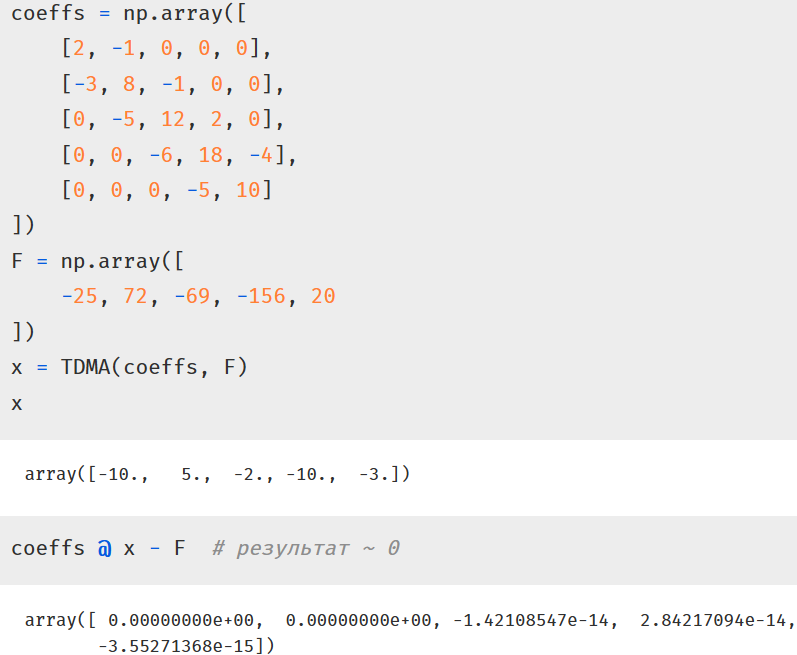
\includegraphics[width=200px,keepaspectratio=true]{TDMA.png}
 
 \caption{Демонстрация работы метода прогонки в среде Jupyter Notebook. Видно, что результат разности левой и правой частей уравнения практически равен 0.}
\end{center}
\end{figure} 

\subsection{Результат численного решения}

\begin{figure}[H]
\centering
\begin{subfigure}{0.4\textwidth}
 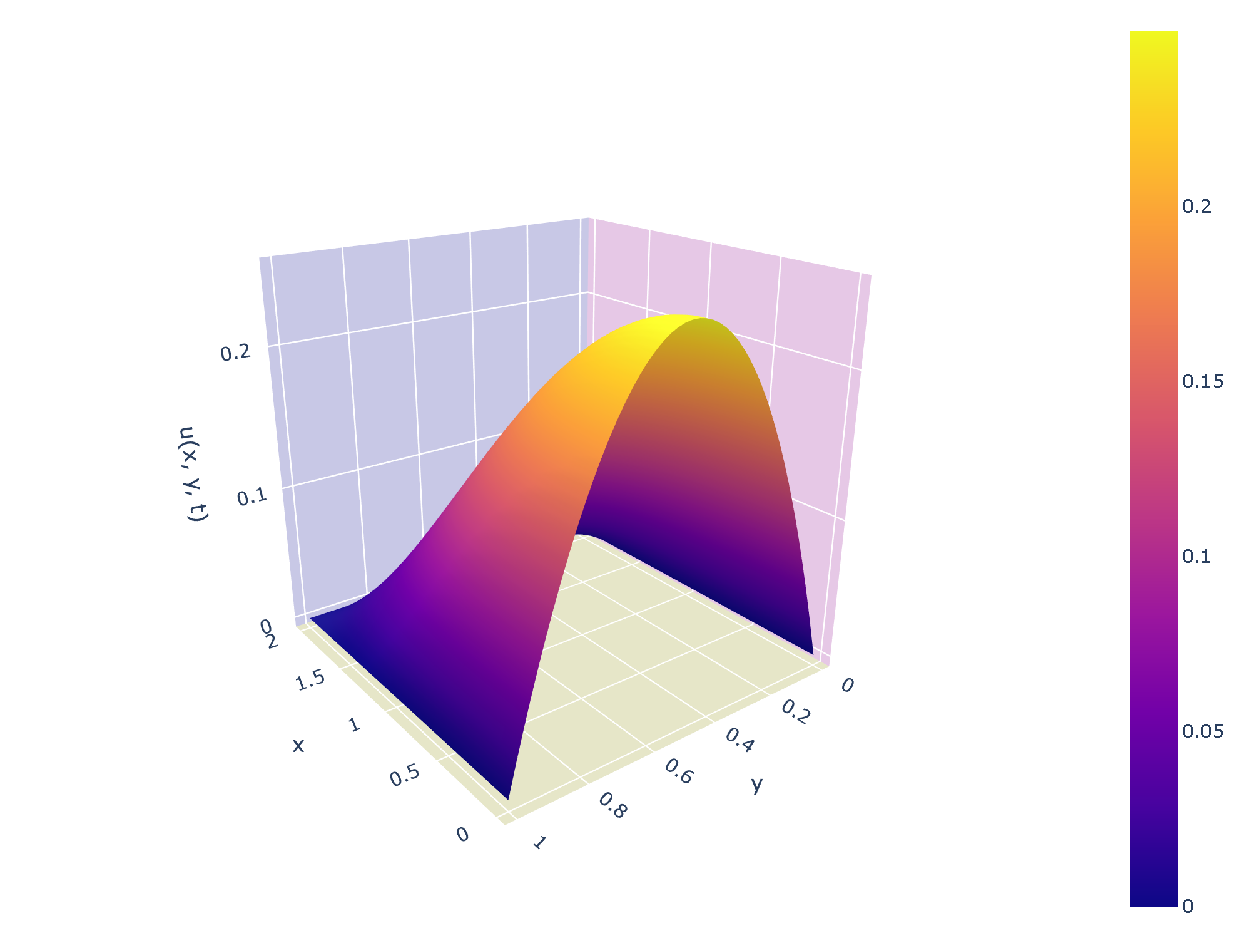
\includegraphics[width=\textwidth,keepaspectratio=true]{start.pdf}
 
 \caption{Начальное состояние}
\end{subfigure}
\begin{subfigure}{0.4\textwidth}
 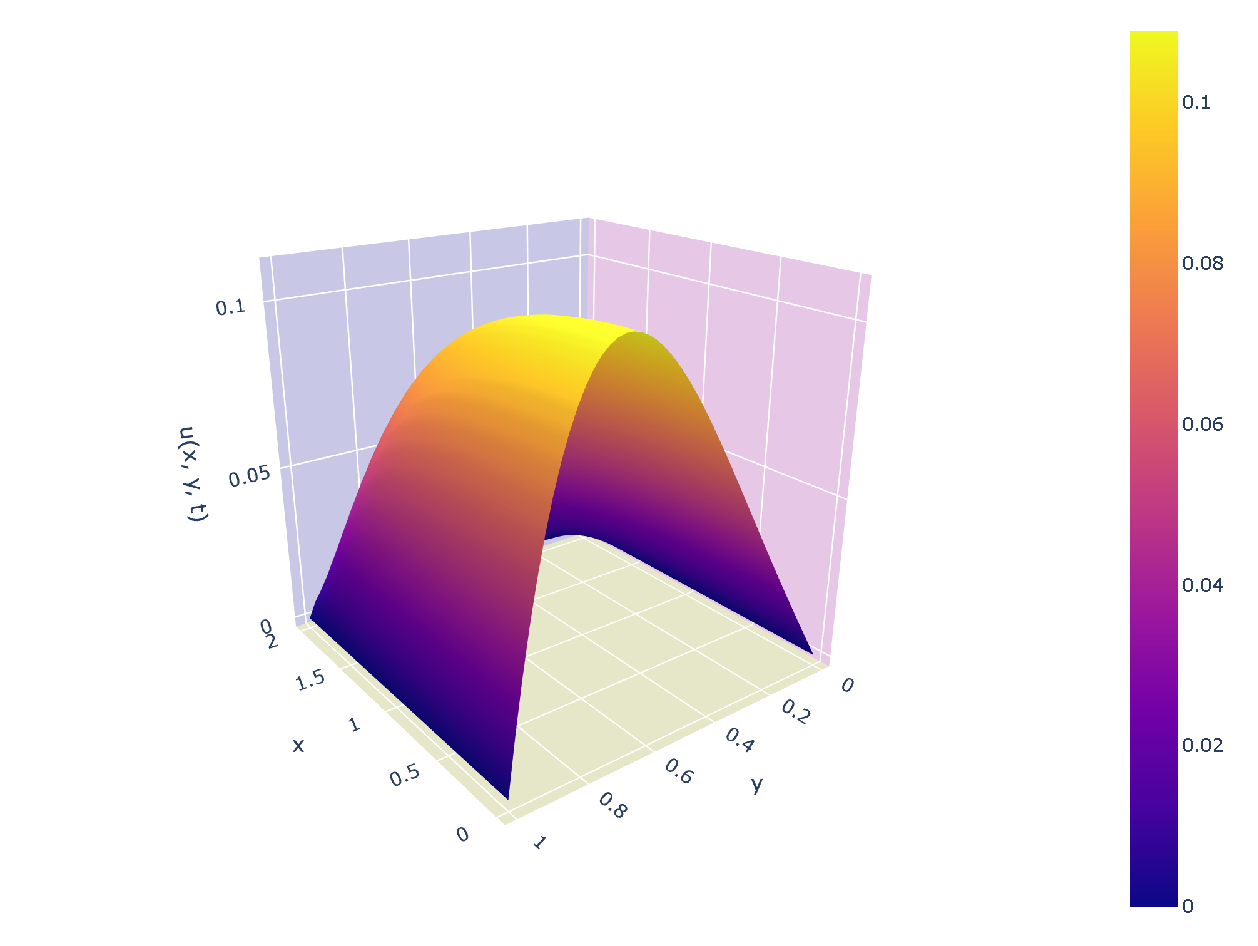
\includegraphics[width=\textwidth,keepaspectratio=true]{middle.pdf}
 
 \caption{Середина времени}
\end{subfigure}
\begin{subfigure}{0.4\textwidth}
 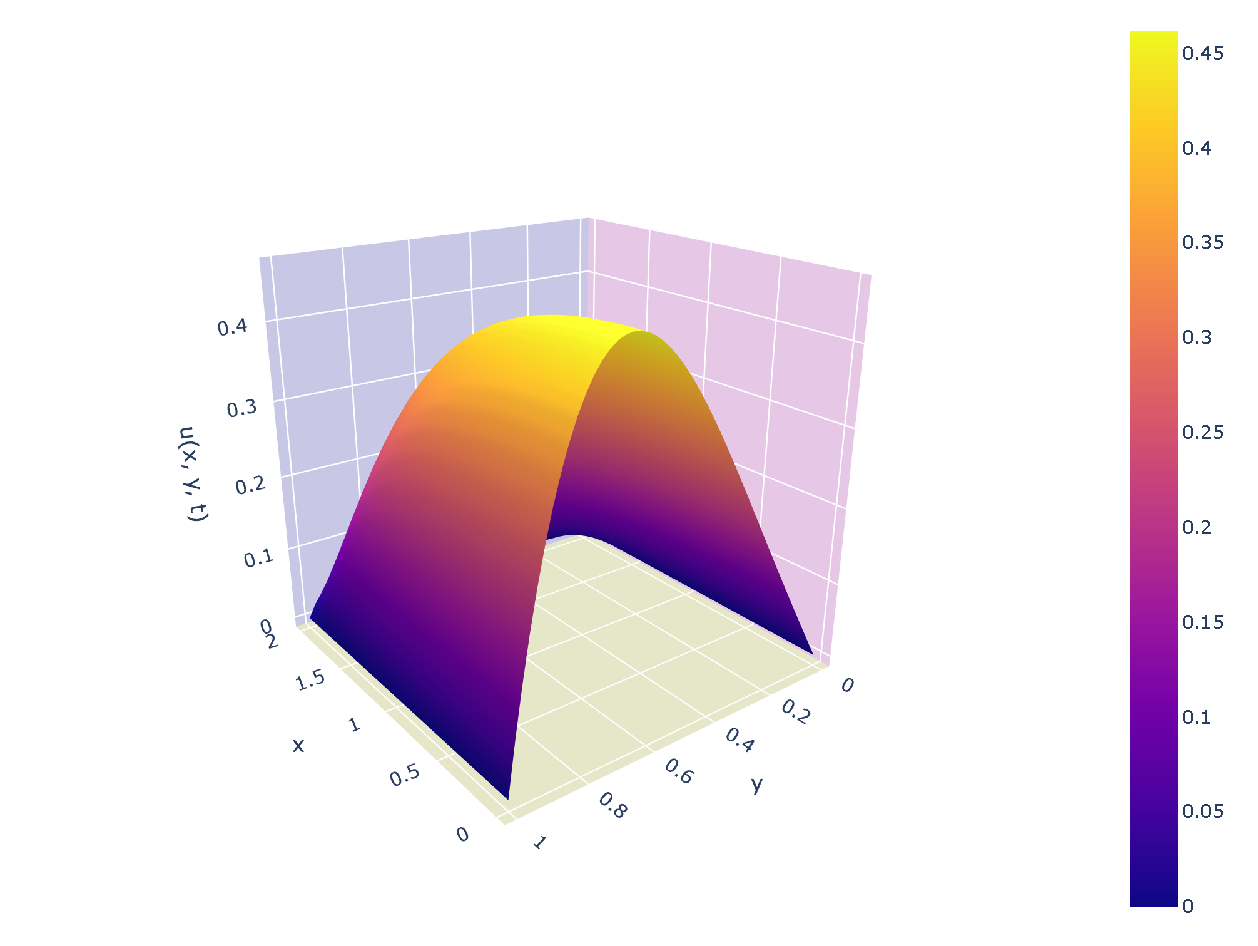
\includegraphics[width=\textwidth,keepaspectratio=true]{end.pdf}
 
 \caption{Конечное состояние}
\end{subfigure}
\caption{Визуализаций эволюции численного решения во времени}
\end{figure}

Анимация эволюции доступна в приложенном .ipynb файле.

\section{Проверка сложности метода переменных направлений}
\begin{figure}[H]
\begin{center}
 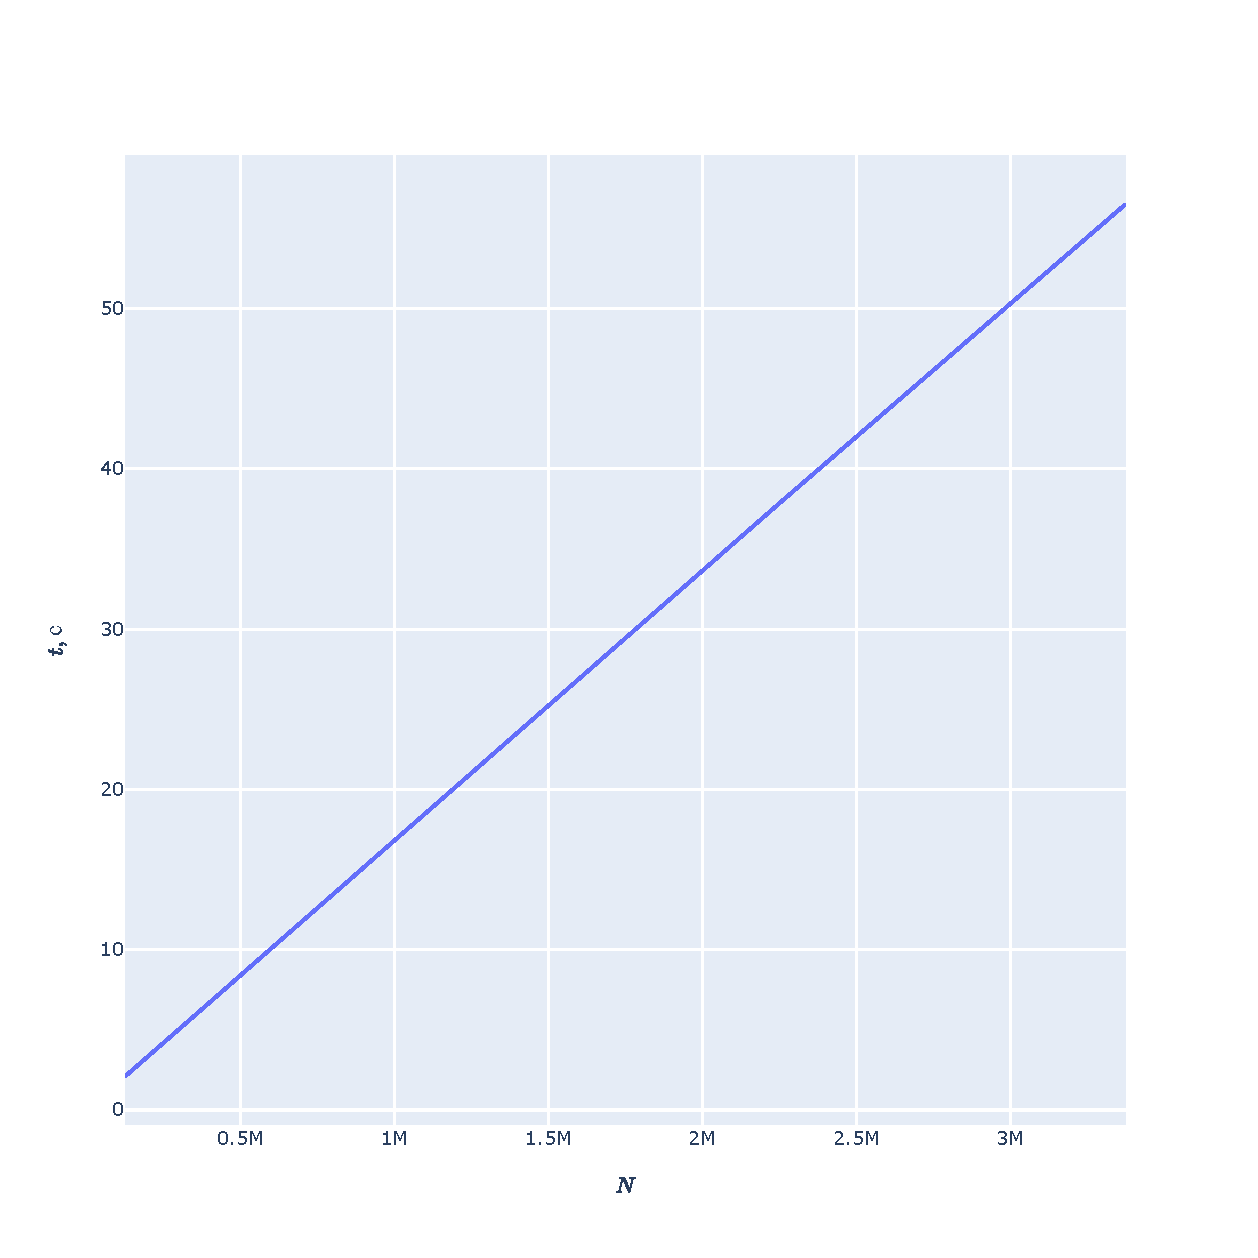
\includegraphics[width=0.7\textwidth,keepaspectratio=true]{performance.pdf}
 
 \caption{График зависимости времени вычисления решения от количества узлов сетки. Видно, что зависимость носит линейный характер.}
\end{center}
\end{figure} 

\section{Заключение}
Было получено численное решение двумерного уравнения тепропроводности. Устойчивость метода подтверждается видом решения. Время вычисления решения пропорционально числу узлов сетки. Таким образом, экспериментально подтверждены теоретические свойства метода переменных направлений.
\end{document} 
